% Options for packages loaded elsewhere
\PassOptionsToPackage{unicode}{hyperref}
\PassOptionsToPackage{hyphens}{url}
\PassOptionsToPackage{dvipsnames,svgnames,x11names}{xcolor}
%
\documentclass[
]{article}
\usepackage{amsmath,amssymb}
\usepackage{iftex}
\ifPDFTeX
  \usepackage[T1]{fontenc}
  \usepackage[utf8]{inputenc}
  \usepackage{textcomp} % provide euro and other symbols
\else % if luatex or xetex
  \usepackage{unicode-math} % this also loads fontspec
  \defaultfontfeatures{Scale=MatchLowercase}
  \defaultfontfeatures[\rmfamily]{Ligatures=TeX,Scale=1}
\fi
\usepackage{lmodern}
\ifPDFTeX\else
  % xetex/luatex font selection
\fi
% Use upquote if available, for straight quotes in verbatim environments
\IfFileExists{upquote.sty}{\usepackage{upquote}}{}
\IfFileExists{microtype.sty}{% use microtype if available
  \usepackage[]{microtype}
  \UseMicrotypeSet[protrusion]{basicmath} % disable protrusion for tt fonts
}{}
\makeatletter
\@ifundefined{KOMAClassName}{% if non-KOMA class
  \IfFileExists{parskip.sty}{%
    \usepackage{parskip}
  }{% else
    \setlength{\parindent}{0pt}
    \setlength{\parskip}{6pt plus 2pt minus 1pt}}
}{% if KOMA class
  \KOMAoptions{parskip=half}}
\makeatother
\usepackage{xcolor}
\usepackage{graphicx}
\makeatletter
\def\maxwidth{\ifdim\Gin@nat@width>\linewidth\linewidth\else\Gin@nat@width\fi}
\def\maxheight{\ifdim\Gin@nat@height>\textheight\textheight\else\Gin@nat@height\fi}
\makeatother
% Scale images if necessary, so that they will not overflow the page
% margins by default, and it is still possible to overwrite the defaults
% using explicit options in \includegraphics[width, height, ...]{}
\setkeys{Gin}{width=\maxwidth,height=\maxheight,keepaspectratio}
% Set default figure placement to htbp
\makeatletter
\def\fps@figure{htbp}
\makeatother
\setlength{\emergencystretch}{3em} % prevent overfull lines
\providecommand{\tightlist}{%
  \setlength{\itemsep}{0pt}\setlength{\parskip}{0pt}}
\setcounter{secnumdepth}{-\maxdimen} % remove section numbering
\usepackage{preamble_ai_project}
\usepackage[backend=bibtex,style=numeric]{biblatex}
\bibliography{references}
\ifLuaTeX
  \usepackage{selnolig}  % disable illegal ligatures
\fi
\IfFileExists{bookmark.sty}{\usepackage{bookmark}}{\usepackage{hyperref}}
\IfFileExists{xurl.sty}{\usepackage{xurl}}{} % add URL line breaks if available
\urlstyle{same}
\hypersetup{
  colorlinks=true,
  linkcolor={Blue},
  filecolor={Maroon},
  citecolor={Blue},
  urlcolor={Blue},
  pdfcreator={LaTeX via pandoc}}

\author{}
\date{}

\begin{document}

\intro{}

\hypertarget{introduction-rappels-thuxe9oriques}{%
\section{1 -- Introduction \& Rappels
théoriques}\label{introduction-rappels-thuxe9oriques}}

Dans ce document, nous approfondirons des techniques de regression
logistique et ``Naive Bayes'' comme outils d'apprentissage superivisés.

Dans le cadre de l'intelligence artificielle et de l'apprentissage
supervisé, la compréhension et la classification précises des données
revêtent une importance capitale. Parmi les diverses méthodologies
existantes, la Régression Logistique et ``Naive Bayes'' se distinguent
par leur efficacité et leur applicabilité dans de nombreux contextes. Ce
document se propose d'étudier ces deux techniques, en mettant l'accent
sur leur mise en œuvre pratique, et leur efficacité comparative dans
divers scénarios.

\hypertarget{ruxe9gression-logistique}{%
\subsection{1.1 -- Régression
Logistique}\label{ruxe9gression-logistique}}

En statistiques, la régression logistique, s'inscrit dans le cadre des
modèles de régression pour les variables binaires.

Ce type de modèle vise à expliquer de manière optimale une variable
binaire, qui représente la présence ou l'absence d'une caractéristique
spécifique, à l'aide d'un ensemble conséquent de données réelles et d'un
modèle mathématique.

Autrement dit, il s'agit de relier une variable aléatoire de Bernoulli,
généralement notée \(y\), aussi appelé ``label'' à un vecteur constitué
de plusieurs variables aléatoires, \((x_1, \ldots, x_K)\), aussi appelés
``features''. \cite{RegressionLogistique2023}.

La régression logistique s'appuie sur un classifeur linéaire
\cite{ClassifieurLineaire2022} i.e.~un classifieur dont la sortie (pour
un vecteur de feature \(x \in \R^n\)) est donnée par:

\[
g(x) = f(\scalproduct{w}{x} + b)
\] où \(w \in \R^n\) est le vecteur de poids, \(b \in \R\) le biais et
\(\scalproduct{.}{.}\) le produit scalair usuel. \(f\) est une fonction
dite de seuillage qui va séparer nos résultats. Un choix commun pour
\(f\) est la sigmoide ou la fonction signe
\cite{ClassifieurLineaire2022}.

Par exemple, dans notre cas, on suppose le modèle suivant: \[
y_i \sim Bernoulli(p_i),\quad p_i = \sigma(\scalproduct{w}{x_i} + b),\quad \sigma(z) = \frac{1}{1 + e^{-z}}
\] où \(x_i\) représente un vecteur (ligne) de \(K\) valeurs pour les
\(K\) features (aussi appelé un \emph{sample}), et \(y_i\) la variable
aléatoire qui représente le label qui leur est associé.

\hypertarget{naive-bayes}{%
\subsection{1.2 -- Naive Bayes}\label{naive-bayes}}

``Naive Bayes'' se présente comme une méthode de classification
probabiliste basée sur le
\href{https://en.wikipedia.org/wiki/Bayes\%27_theorem}{théorème de
Bayes}, caractérisée par l'adoption d'une hypothèse d'indépendance forte
entre les features (attributs), qualifiée de ``naïve''.\\
Plus simplement, le classifieur est classifié de ``naïf'' car il part du
principe que chaque feature (attribut) est indépendante des autres et a
un poid égal quant à la probabilité qu'un point appartienne à une
classe.

Ce model est dit génératif contrairement à la regression logistique
étant considéré comme ``méthode discriminante''
\cite{ClassifieurLineaire2022} et consiste à modéliser les probabilités
conditionnelles \(P(X | classe)\) pour chaque classe \(y\) et vecteur de
features \(X\) afin de trouver celle qui maximise cette probabilité.

En d'autres termes, le problème revient à trouver, pour des attributs
\(X_1, \ldots, X_k\), la classe \(\tilde{y}\) telle que:

\[
\tilde{y} = \text{arg}\max_{Y \in \mathcal{Y}} \left[\  P(Y) \prod_{k = 1}^K{P(X_k | Y)}\  \right]
\]

Citation Test: \cite{LinearModels}

\hypertarget{muxe9thodologie}{%
\section{2 -- Méthodologie}\label{muxe9thodologie}}

\hypertarget{choix-du-dataset-outils-utilisuxe9s}{%
\section{2.0 -- Choix du dataset \& outils
utilisés}\label{choix-du-dataset-outils-utilisuxe9s}}

Pour la suite de ce projet les outils suivants ont été utilisés dans
chaque parties:

\begin{itemize}
\tightlist
\item
  \href{https://www.python.org/}{python}
\item
  \href{https://numpy.org/}{numpy}
\item
  \href{https://scikit-learn.org/stable/}{sklearn}
\item
  \href{https://matplotlib.org/}{matplotlib}
\item
  \href{https://github.com/uci-ml-repo/ucimlrepo}{ucmilrepo}
\end{itemize}

Le package \texttt{ucmilrepo} a été utilisé pour charger les données de
notre dataset depuis la base de donnée du
\href{https://archive.ics.uci.edu/ml/index}{UC Irvine Machine Learning
Repository}.

Le dataset que nous avons choisi est le fameux dataset ``Iris''
\cite{r.a.fisherIris1936}, un des plus anciens et connus dataset de
classification. Il contient 150 observations de 3 espèces différentes
d'iris (Iris setosa, Iris virginica et Iris versicolor) avec 4 features
(longueur et largeur des sépales et pétales).

Voici un aperçu des points-clés du dataset:

\begin{figure}
\centering
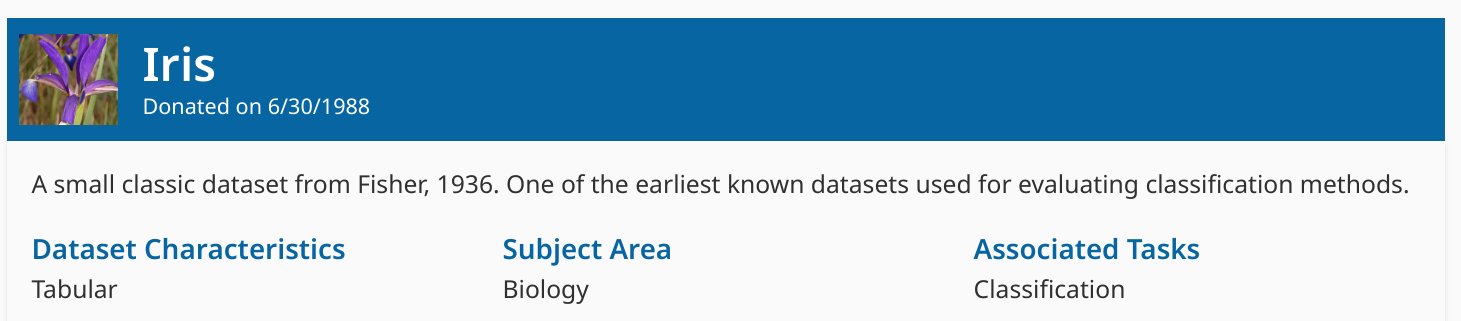
\includegraphics[width=0.8\textwidth,height=\textheight]{../res/iris_img.png}
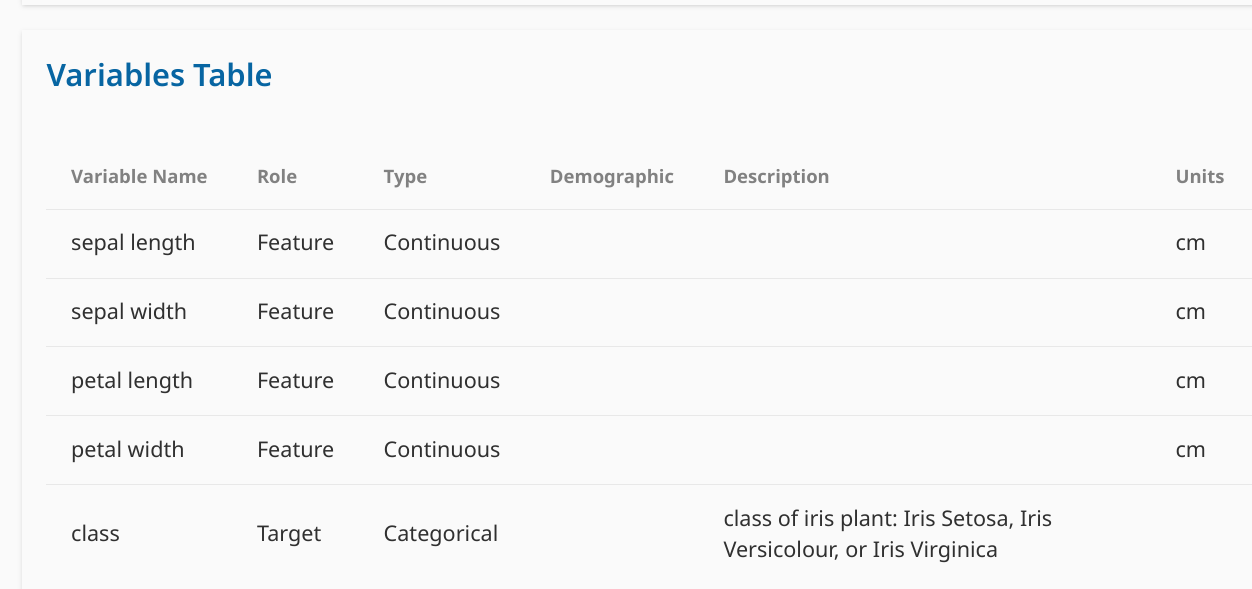
\includegraphics[width=0.8\textwidth,height=\textheight]{../res/iris_table.png}
\caption{Iris descriptive table}
\end{figure}

Le label que nous allons prédire sera donc \emph{class}, i.e.~l'espèce
de l'iris.

\newpage

\hypertarget{gradient-descent}{%
\subsection{2.1 -- Gradient Descent}\label{gradient-descent}}

Dans cette section, une implémentation de la ``descente en gradient'' a
été réalisée. La fonction a la signature suivante

\begin{lstlisting}
  def gradient_descent(df, params: NDArray, alpha: float, num_iters: int) -> NDArray:  
\end{lstlisting}

Elle calcule de manière itérative le(s) paramètre(s) \code{params} qui
minimisent la fonction dont \texttt{df} est le gradient avec un ``taux
de convergence'' \code{alpha}.

La fonction a été testé avec la fonction \code{scipy.optimize.fmin}
\cite{ScipyOptimizeFmin} de la librairie \texttt{scipy} sur la fonction
suivante: \[
f(x) = x * \cos(\pi  (x + 1))
\]

avec différents \(x_0 \in \{-\pi, 0, \pi\}\) (valeur initiale de
\code{params}, i.e.~\texttt{NDArray} avec D=0).

Les minimas locaux trouvés par les deux fonctions sont les suivants:

\begin{figure}
\centering
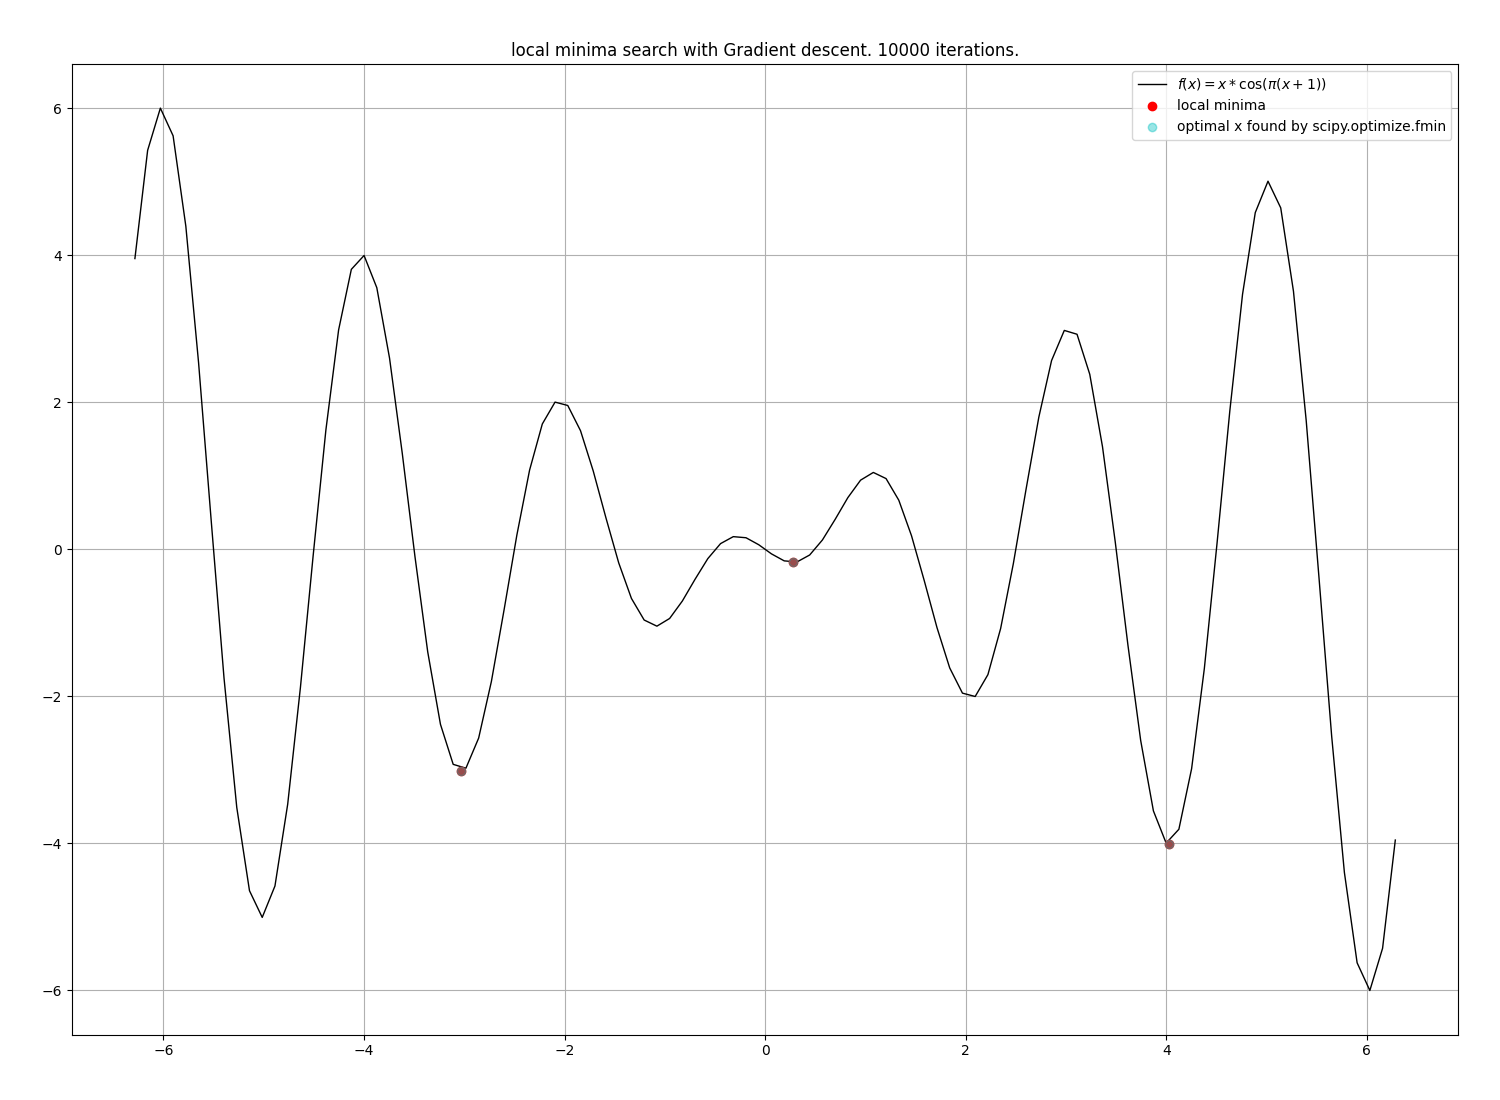
\includegraphics[width=1\textwidth,height=\textheight]{../res/3.1_gradient_descent_minima.png}
\caption{minimas locaux\_gradient descent}
\end{figure}

Ce résultat illustre bien 2 choses: la première est que l'implémentation
de la descente en gradient fonctionne correctement puisque pour chaque
points trouvé par notre fonction est confondu avec celui trouvé par la
fonction de scipy (c'est ce qui donne cette teinte ``grise''). La
deuxième est que la ``qualité'' du minima local (i.e.~la distance avec
le minima globale) dépend fortement de la valeur initiale et ce pour les
deux fonctions.

\newpage{}

\hypertarget{ruxe9gression-logistique-1}{%
\subsection{2.2 -- Régression
Logistique}\label{ruxe9gression-logistique-1}}

\begin{center}\rule{0.5\linewidth}{0.5pt}\end{center}

\hypertarget{naive-bayes-1}{%
\subsection{2.3 -- Naive Bayes}\label{naive-bayes-1}}

Dans section, une implémentation d'un classifieur bayesien (naive bayes)
a été réalisée. La fonction de prédictition a la signature suivante:

\begin{lstlisting}
    #  TODO
\end{lstlisting}

et calcule la classe qui maximise la probabilité conditionnelle définie
en section \href{#naive-bayes}{1.2}.

Dans cette impléntation, étant données que toutes nos features sont
continues, nous avons considéré que \emph{sepal length}, \emph{sepal
width}, \emph{petal length} et \emph{petal width} seront représenté
comme 4 variables aléatoires \(X_0, \cdots, X_3\) suivant 4 lois
normales normales de paramètre \((\mu_k, \sigma_k)\).

C'est à dire: \[
X_k \sim \mathcal{N}( \mu_k, \sigma_k) \qquad \qquad k \in \iitv{0, 3}
\]

\newpage{}

\hypertarget{ruxe9sultats}{%
\section{3 -- Résultats}\label{ruxe9sultats}}

\printbibliography[heading=bibintoc, title={Références}]

\begin{itemize}
\tightlist
\item
  TODO: ajouter les autres références des documentations utilisées
\end{itemize}

\end{document}
